\documentclass[a4paper,11pt, twocolumn]{article}
\usepackage[margin=0.8in]{geometry}
\usepackage{xcolor}
\usepackage{graphicx} %package to manage images
\graphicspath{ {./images/} }
\usepackage{float}
\usepackage{tabularx}

\title{1.2.4 Types Of Programming Language}
\author{Revision sheet}
\date{}

\usepackage{fancyhdr}
\pagestyle{fancy}
\fancyhead{} % clear all header fields
\renewcommand{\headrulewidth}{0pt} % no line in header area
\fancyfoot{} % clear all footer fields
\renewcommand{\footrulewidth}{0.4pt}
\fancyfoot[C]{\thepage} % page number in centre of the page
\fancyfoot[R]{\footnotesize Thomas Boxall \\ } % right hand footer has author name on top line and images reference on bottom line
\fancyfoot[L]{\footnotesize 1.2.4 Types Of Programming Language \\ Revision sheet} % left hand footer has title of document on top line and 'Revision Sheet' on bottom line


\begin{document}

\maketitle
\thispagestyle{fancy}

% CONTENTS OF THE REVISION SHEET HERE
\section{Programming Paradigms}
A \textit{programming paradigm} is a style of programming. Different languages use different paradigms, some languages support more than one paradigm. Different problems require different paradigms.
\subsection{Procedural}
This paradigm, is where you have a series of instructions that tell the computer what to do with the input in order to solve the problem. They are easy to learn and applicable to a wide variety of problems. Structured programming is a type of procedural programming which uses sequence, selection, iteration and recursion. It uses modular techniques to split large programs into manageable chunks. Languages include Python and Pascal.
\subsection{Object-Oriented}
This paradigm was developed to make possible to abstract details of implementation away from the programmer, making code reusable and easy to maintain. To a great extent, it is taking over from procedural programming. Languages include Java, Python and Delphi.
\subsection{Declarative}
This paradigm is where the programmer writes statements that describe the problem to be solved, and the language implementation decides the best way of solving it. Languages include SQL which is used to query databases.
\subsection{Functional}
This paradigm uses functions as the fundamental building block, statements are written as a series of functions which accept inputs and return outputs. Languages include Haskell, Python, C\# and Java.

\section{Procedural Languages}
This has built in data types (eg, integer, real, floating point, character, Boolean and string) and some built in data structures (array and record). Programmers can define their own abstract data structures (eg, queue, stack, tree). There are a number of different ways in different languages that these abstract data structures can be implemented. 

\section{Object Oriented Languages}
OO Languages are based off of `classes', which we define as a description of what the data looks like and what the data can do. Instances of the class are then created and used, these are called `objects'. OO programming requires thinking in terms of objects that wil carry out teh required tasks, rather than thinking about the data structures or algorithms. Objects could be cat, dog, plate, car, etc. There can be multiple instances of the same class at the same time in a program.
\subsection{Inheritance}
The following explanation will make use of the very simple class diagram shown below.
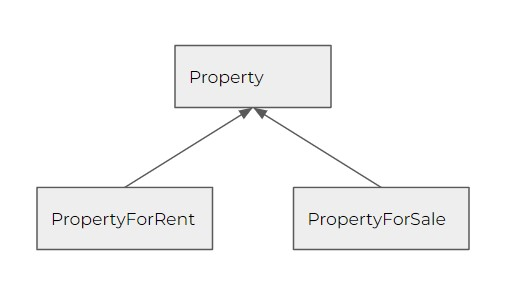
\includegraphics[width=0.45\textwidth]{basicClassDiagram.jpg}
The `superclass' \verb|Property| contains a number of attributes and methods. The `subclasses' \verb|PropertyForRent| and \verb|PropertyForSale| inherit all of the class \verb|Property| methods and attributes. They can also have their own.
\subsection{Polymorphism}
Polymorphism refers to the programming languages ability to process objects differently depending on their class. Methods declared with the same name will be taken from the closest to the class which the object is an instance of. This means that if a method is given the same name in both \verb|Property| and \verb|PropertyForSale| within \verb|PropertyForSale|, the method used will be the one declared within itself. 
\subsection{Encapsulation}
This binds together the attributes and the methods that manipulate the data so that the data is protected. Generally attributes will be declared as \verb|private|, meaning they are only accessible within the object; then \verb|get| and \verb|set| methods will be used to get and set the attribute. These methods can contain validation.
\subsection{Advantages Of The Object-Oriented Paradigm}
The OO methodology forces designers to go through an extensive planning phase, which makes for better designs with fewer weaknesses; encapsulation; once an object has been created, knowledge of its inner workings are not necessary for a programmer to use it; new objects can easily be created with smaller differences to existing ones; objects that are already defined can be re-used in many projects; OOP provides a good framework for code libraries; OOP is much easier to maintain because of its modular structure. 

\section{Assembly Language}
Assembly language code uses mnemonics to represent the operation codes and addresses. The assembler translates the assembly language program into machine code for execution. 
\subsection{Little Man Computer Instructions}
\begin{table}[H]
    \centering
    \begin{tabularx}{0.45\textwidth}{ccc|X}
     &  &  & Instruction \\
     \hline
     & LDA & xxx & Load xxx to the accumulator \\
     & STA & xxx & Store accumulator to xxx \\
     & ADD & xxx & Add xxx to accumulator \\
     & SUB & xxx & Subtract xxx from accumulator \\
     & INP &  & Input from keyboard to accumulator \\
     & OUT &  & Output from accumulator to display \\
     & HLT &  & End program (Halt) \\
     & BRZ & xxx & Branch to xxx if accumulator is zero \\
     & BRP & xxx & Branch to xxx if accumulator is greater than or equal to zero \\
     & BRA & xxx & Branch always to xxx \\
    xxx & DAT & val & Declares variable called xxx
    \end{tabularx}
\end{table}

\section{Memory Addressing}
There are a number of different ways to locate data and instructions in memory. Memory addressing modes determine the method used within the program to access data either from within the CPU or external RAM. Some memory addressing modes can control program flow. Low level languages allow the programmer to directly choose which method they want to use. 
\subsection{Immediate Addressing}
The data to be used is hard-coded into the instruction itself, this makes it fast as it doesn't involve memory at all.
\subsection{Direct or Absolute Addressing}
The code refers directly to a memory location. This is fast but unreliable (as data won't always be in the same location). This is used in applications where the computer is only running a single program.
\subsection{Indirect Addressing}
The address of the data is held in an intermediate location so that the address is first `looked up' and then used to locate the data itself.
\subsection{Indexed Addressing}
The address is determined by adding an offset to a base address. Very often, chunks of data are stored as complete blocks in memory (eg, arrays). It is fast and excellent for manipulating data structures such as arrays. 


\end{document}
- need for and characteristics of a variety of programming paradigms
- procedural languages
- assembly language (incl. syntax)
- modes of addressing memory (immediate, direct, indirect and indexed)
- OO languages with an understanding oof classes, objects methods, attributes, inheritance, encapsulation and polymorphism.